\documentclass[a4paper]{article}

\usepackage{cite}%多个文献引用
\usepackage{graphicx}
\usepackage{array}%调节表格行高
\usepackage{multirow,makecell}%多行表格
\usepackage{tabularx}%表格固定列宽
\usepackage{subfigure}
\usepackage{titlesec}%标题格式设置
\usepackage{amsmath}
\usepackage{amssymb}
\usepackage{tabularx}
\usepackage{makecell}
\usepackage{geometry}
\usepackage{float}
\usepackage{setspace}%行距包
\usepackage{siunitx}
\usepackage{mdwlist}
\usepackage{tabu}
\usepackage{enumerate}

\geometry{top=1.54cm,bottom=2.54cm,left=2.5cm,right=2.5cm}


\begin{document}
\begin{center}
\bf\Large
EE 105 Feedback Control Systems\par
Department of Electrical and Computer Engineering\par
Tufts University Fall 2018\par
Homework \#7\par   
\end{center}
\begin{table}[H]
\begin{center}
\begin{tabular*}{\textwidth}{@{\extracolsep{\fill}}lcr}
Name: {\it Shang Wang} &Student ID: {\it 1277417} &E-mail: {\it shang.wang@tufts.edu}\\
\hline
\end{tabular*}
\end{center}
\end{table}

\section{Problem 1}
\subsection{Part A} 
The transfer function is:
$$
L(s) = \frac{1}{s+1}
$$
\begin{figure}[H]
\centering
\begin{minipage}[t]{0.48\textwidth}
\centering
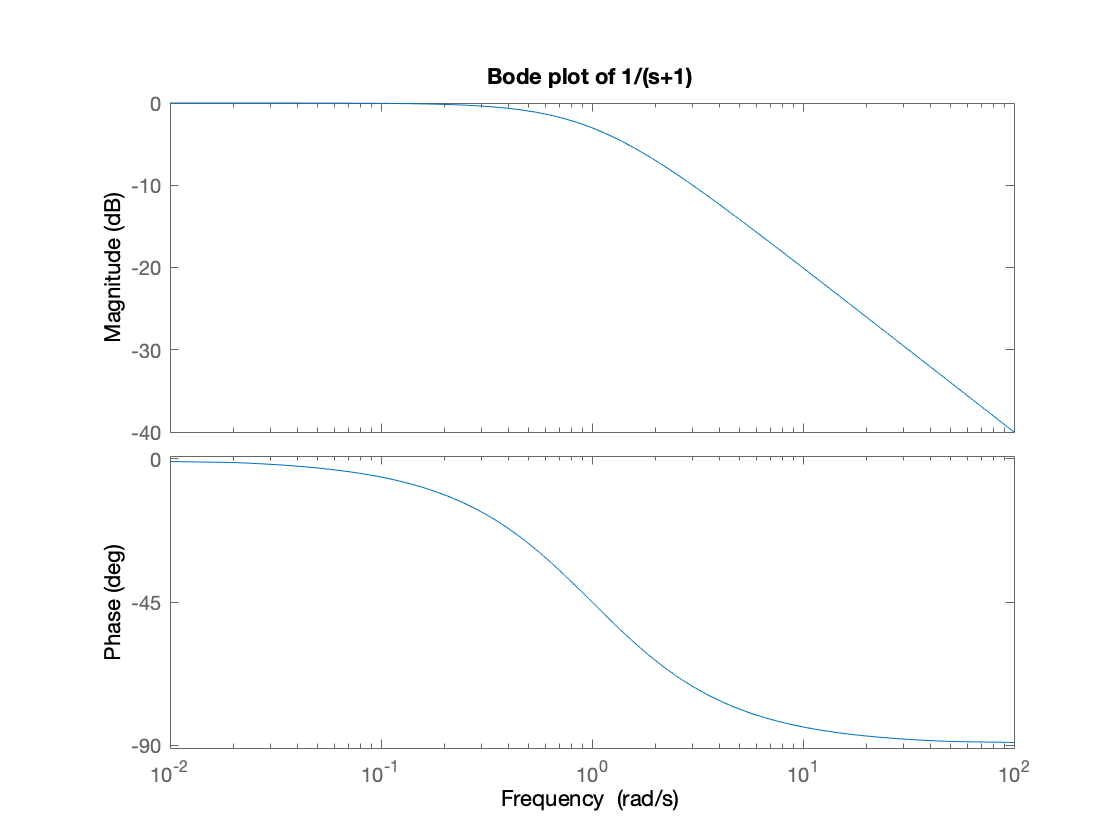
\includegraphics[width=\textwidth]{pic/1.png}
\end{minipage}
\begin{minipage}[t]{0.48\textwidth}
\centering
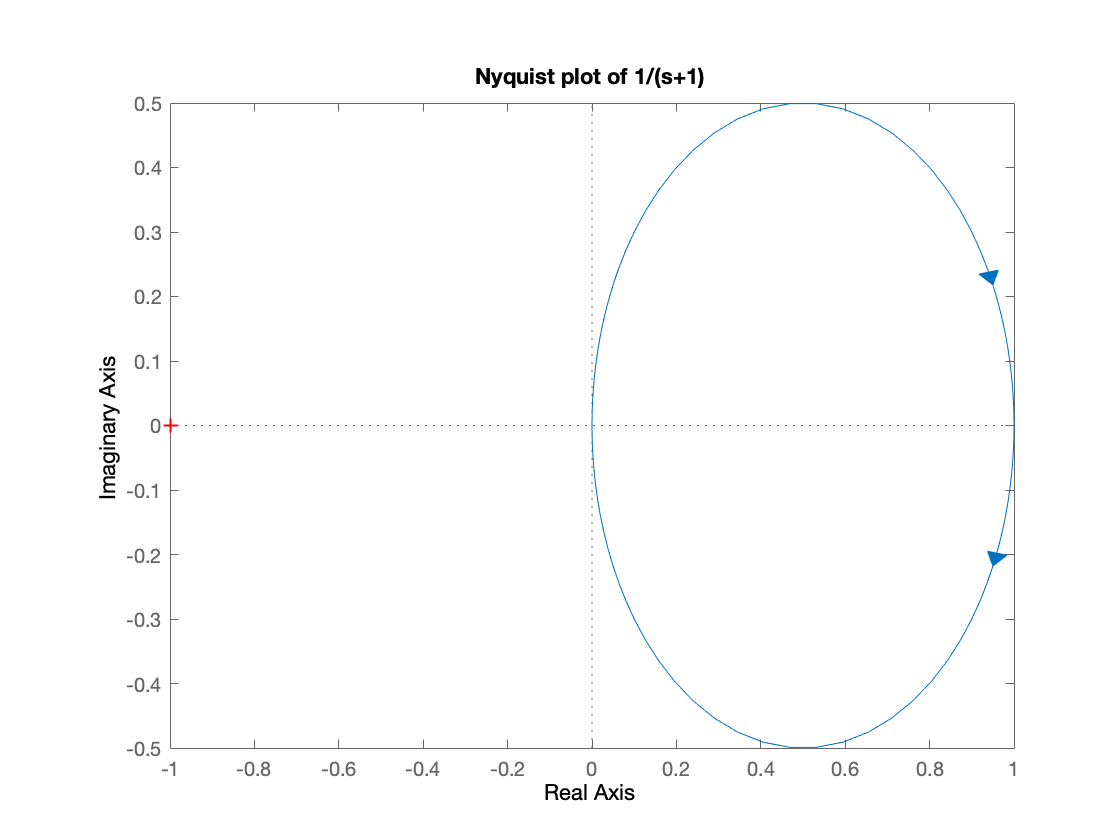
\includegraphics[width=\textwidth]{pic/2.png}
\end{minipage}
\end{figure}
It's stable even if crank $K$ up to infinity.

\subsection{Part B} 
The transfer function is:
$$
L(s) = \frac{10}{(s+1)(s+3)}
$$
\begin{figure}[H]
\centering
\begin{minipage}[t]{0.48\textwidth}
\centering
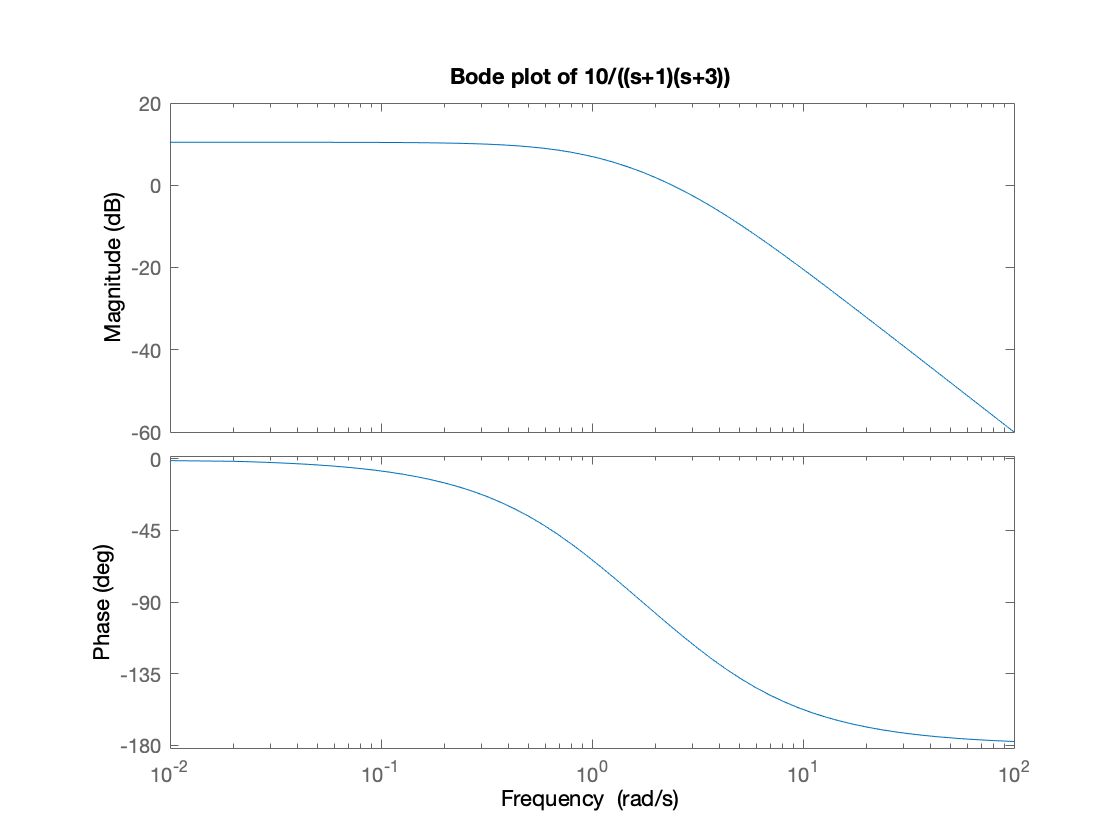
\includegraphics[width=\textwidth]{pic/3.png}
\end{minipage}
\begin{minipage}[t]{0.48\textwidth}
\centering
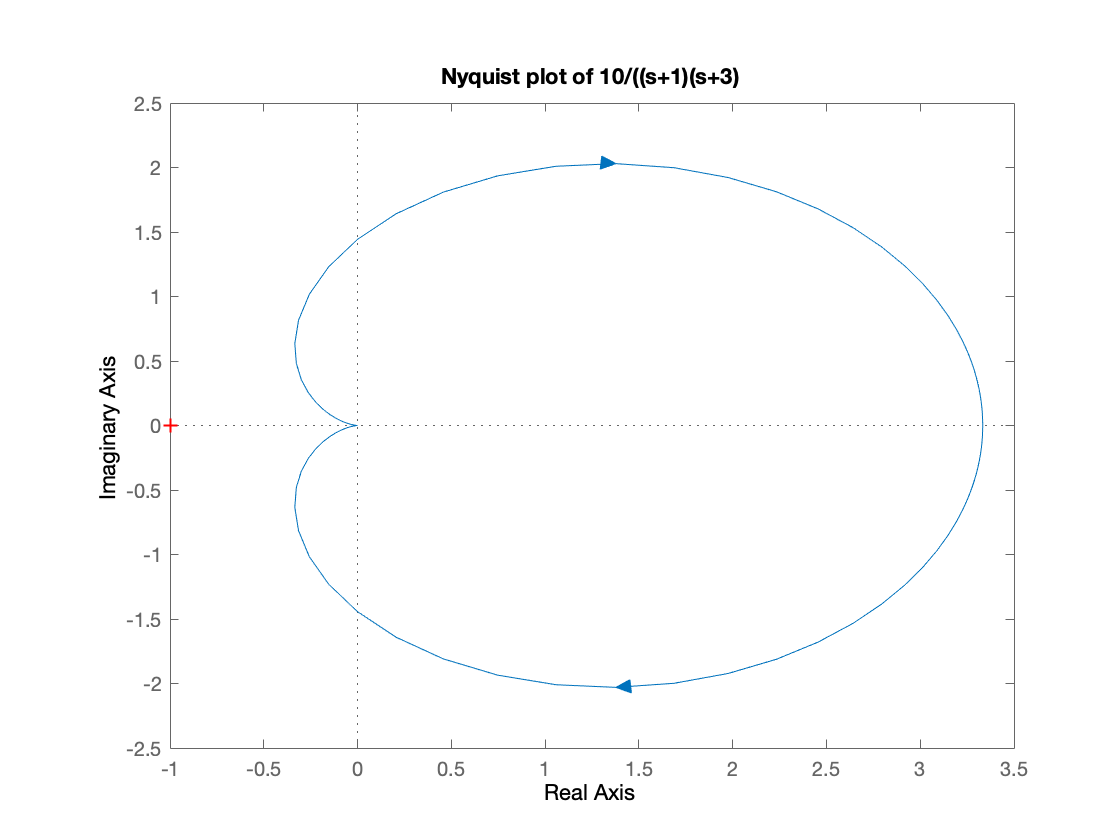
\includegraphics[width=\textwidth]{pic/4.png}
\end{minipage}
\end{figure}
It's stable even if crank $K$ up to infinity.

\subsection{Part C} 
The transfer function is:
$$
L(s) = \frac{50}{(s+1)(s+3)(s+5)}
$$
\begin{figure}[H]
\centering
\begin{minipage}[t]{0.48\textwidth}
\centering
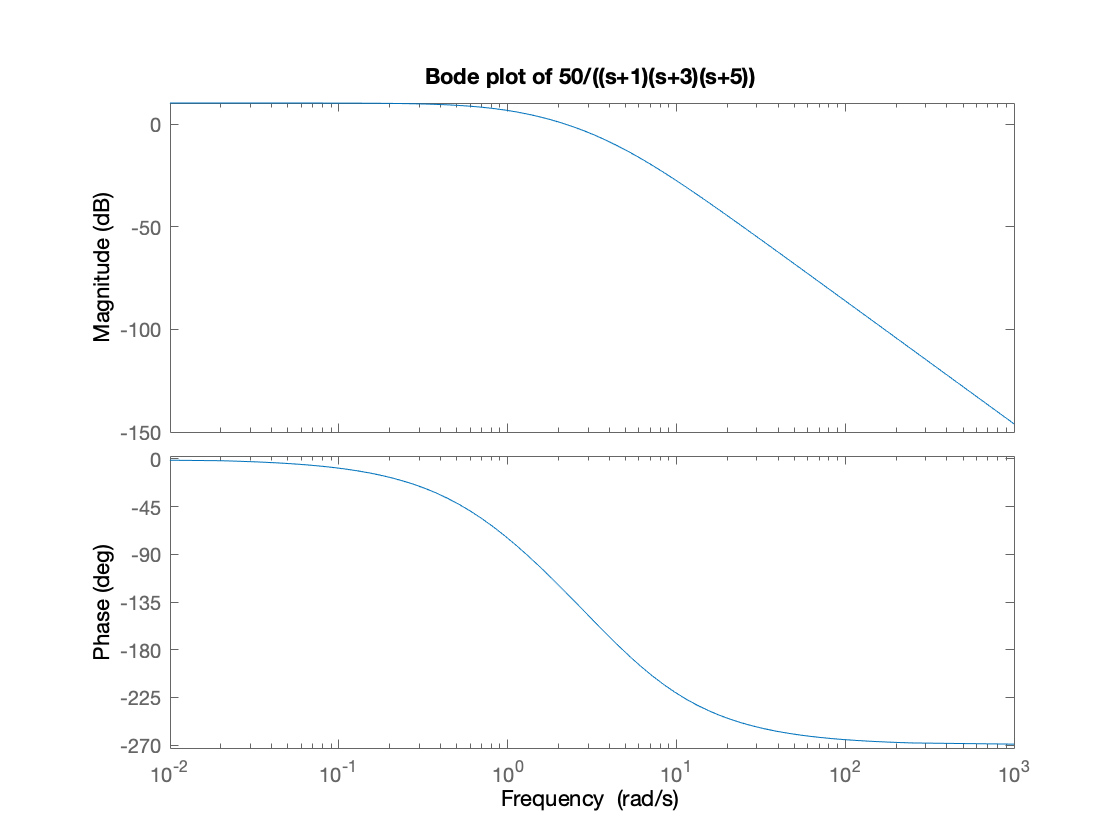
\includegraphics[width=\textwidth]{pic/5.png}
\end{minipage}
\begin{minipage}[t]{0.48\textwidth}
\centering
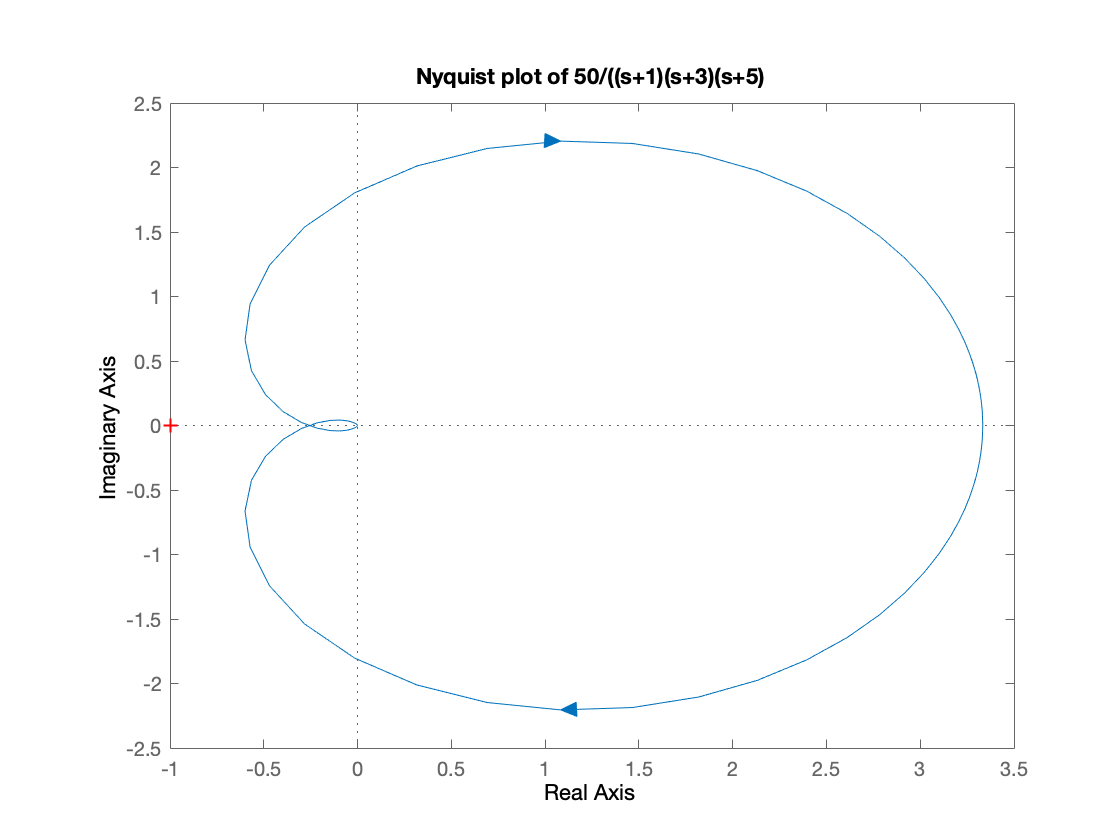
\includegraphics[width=\textwidth]{pic/6.png}
\end{minipage}
\end{figure}
It's stable. But if give an additional gain of $4$, the system will be unstable.

\subsection{Part D} 
The transfer function is:
$$
L(s) = \frac{10}{(s+1)^4}
$$
\begin{figure}[H]
\centering
\begin{minipage}[t]{0.48\textwidth}
\centering
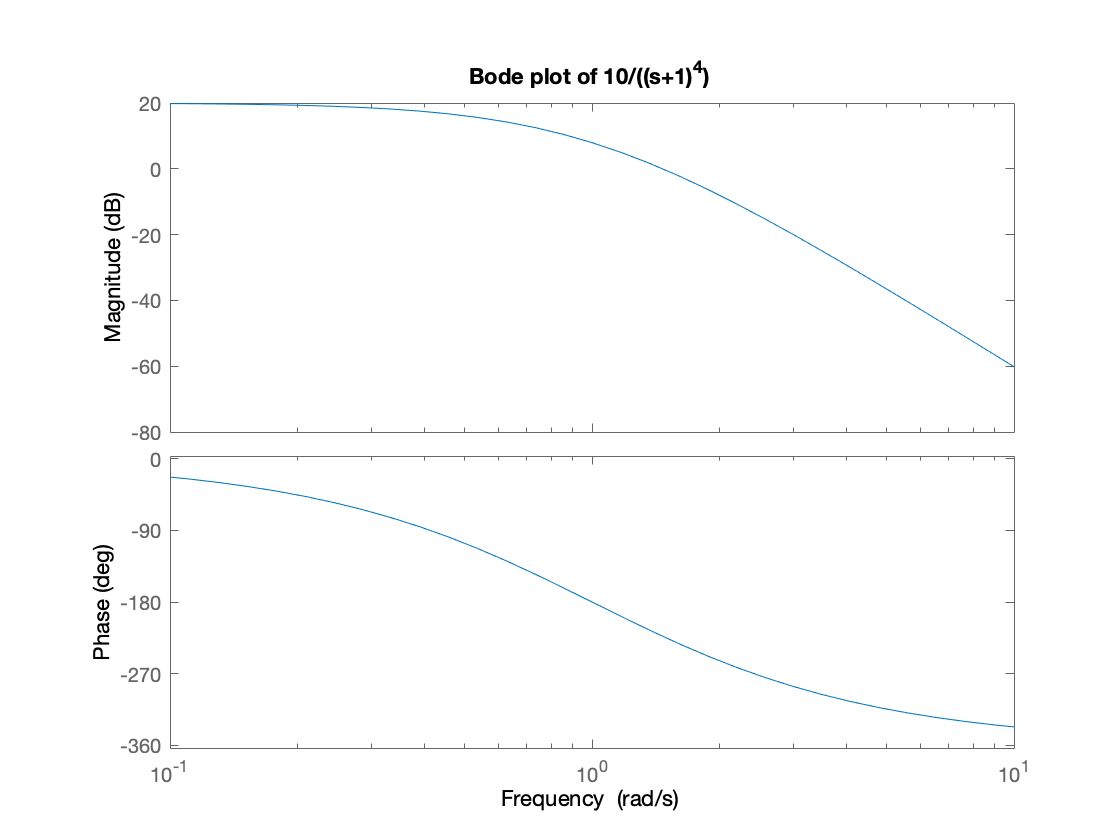
\includegraphics[width=\textwidth]{pic/7.png}
\end{minipage}
\begin{minipage}[t]{0.48\textwidth}
\centering
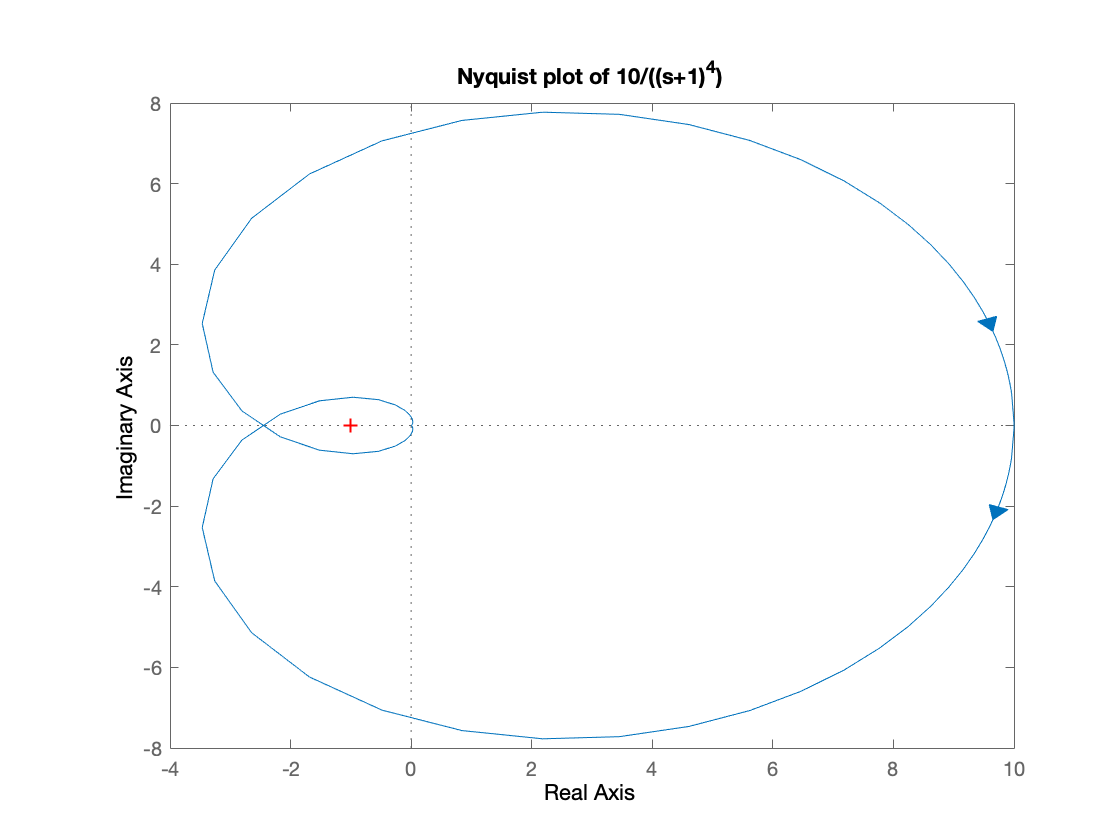
\includegraphics[width=\textwidth]{pic/8.png}
\end{minipage}
\end{figure}
It's unstable. But if give an additional gain of $0.41$, the system will be stable.

\subsection{Part E} 
The transfer function is:
$$
L(s) = \frac{50(s+0.1)}{(s+1)(s+3)(s+5)}
$$
\begin{figure}[H]
\centering
\begin{minipage}[t]{0.48\textwidth}
\centering
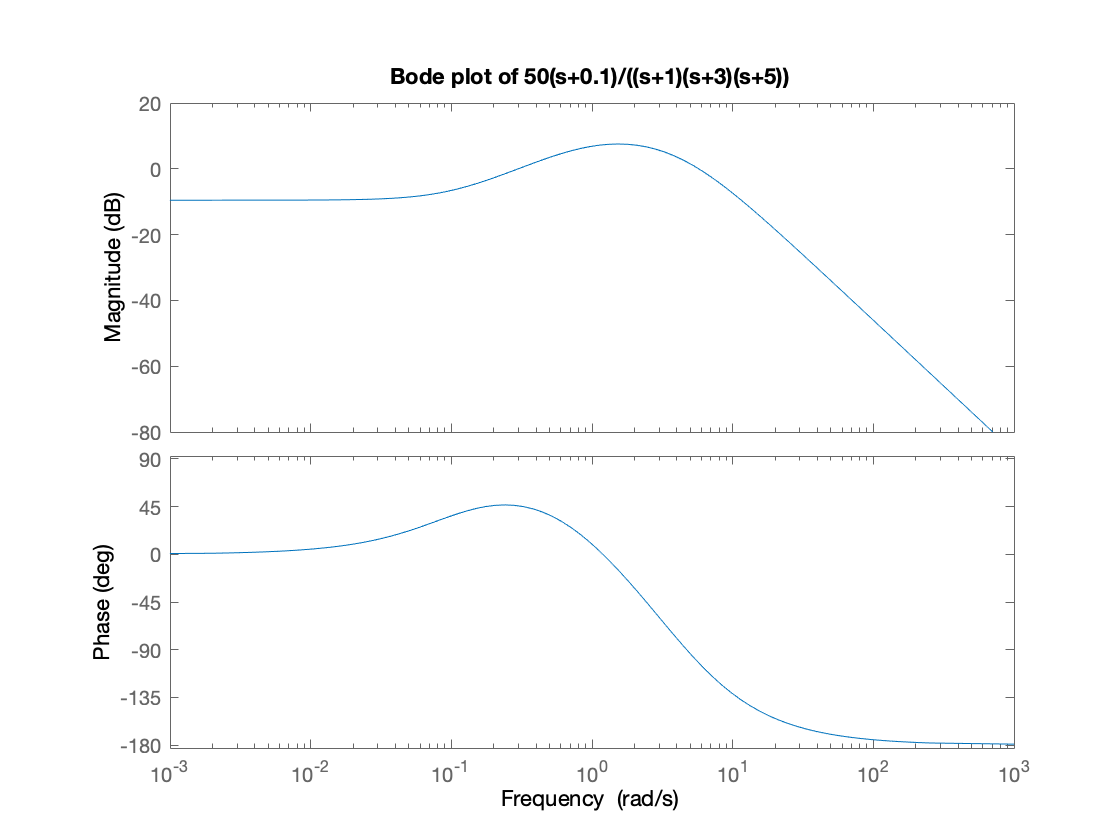
\includegraphics[width=\textwidth]{pic/9.png}
\end{minipage}
\begin{minipage}[t]{0.48\textwidth}
\centering
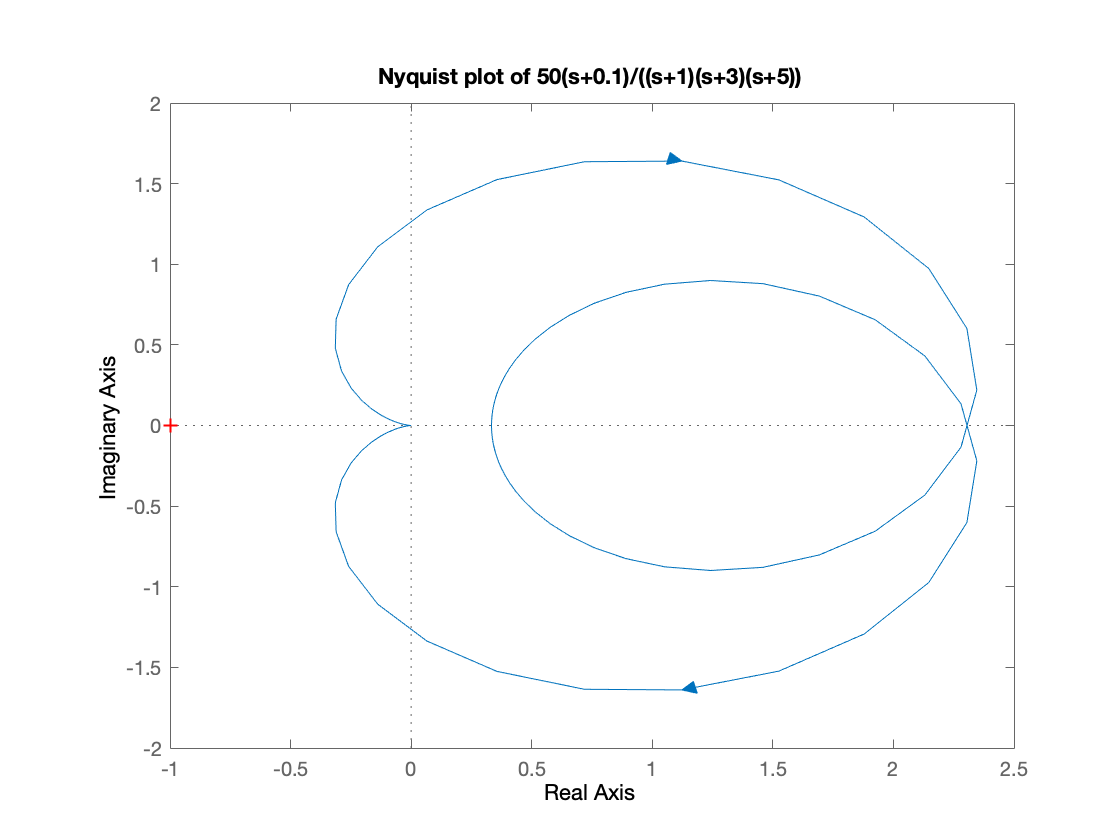
\includegraphics[width=\textwidth]{pic/10.png}
\end{minipage}
\end{figure}
It's stable even if crank $K$ up to infinity.

\subsection{Part F} 
The transfer function is:
$$
L(s) = \frac{s+1}{s^2+s+1}
$$
\begin{figure}[H]
\centering
\begin{minipage}[t]{0.48\textwidth}
\centering
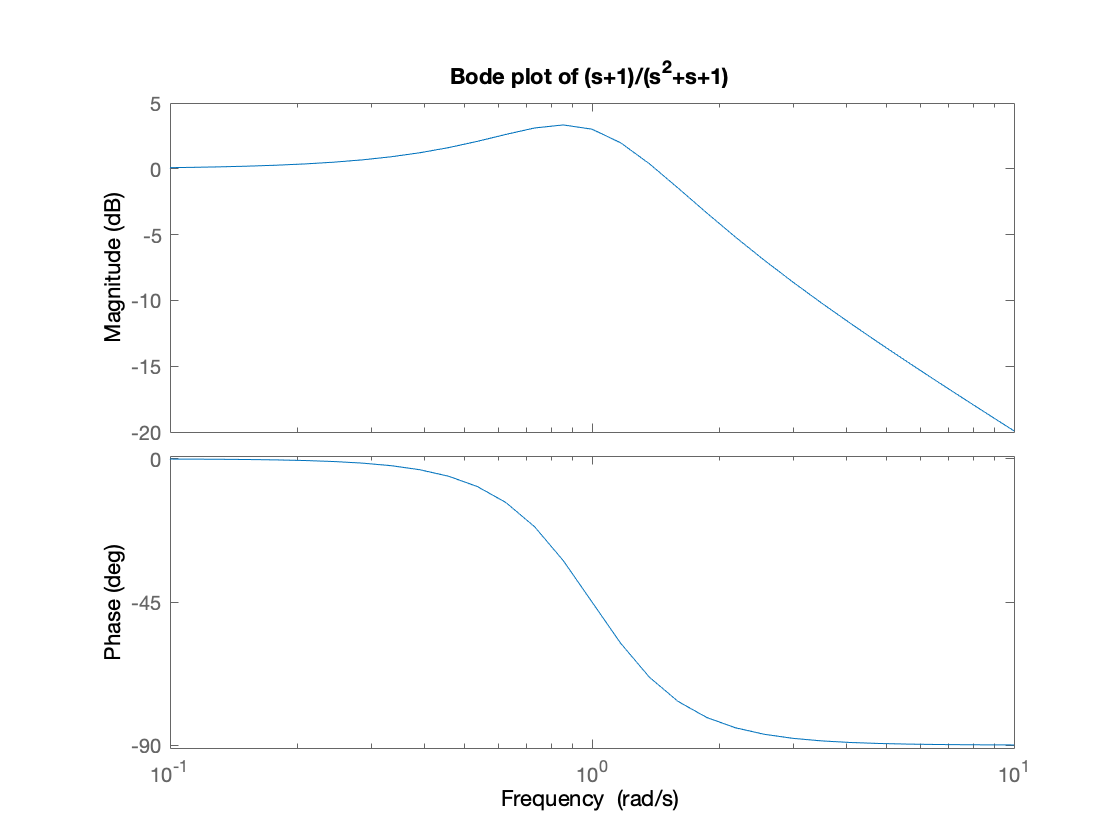
\includegraphics[width=\textwidth]{pic/11.png}
\end{minipage}
\begin{minipage}[t]{0.48\textwidth}
\centering
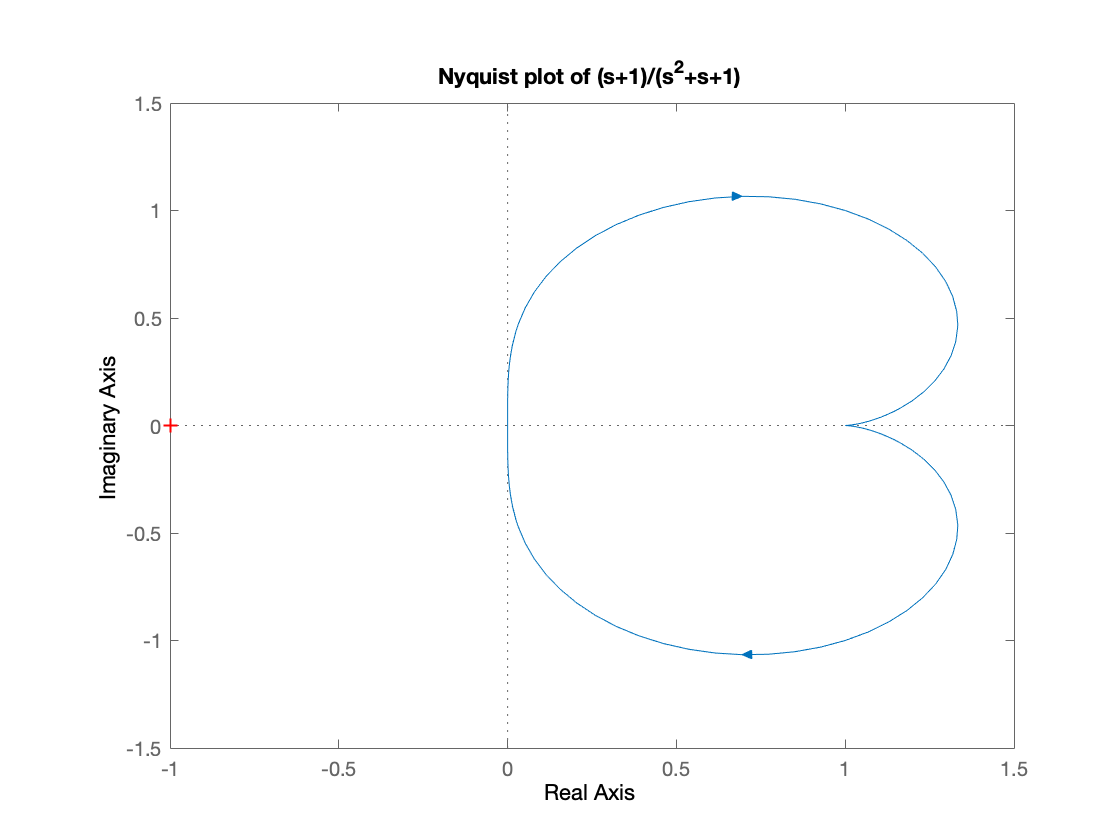
\includegraphics[width=\textwidth]{pic/12.png}
\end{minipage}
\end{figure}
It's stable even if crank $K$ up to infinity.


\subsection{Part F} 
The transfer function is:
$$
L(s) = \frac{s+1}{s^2+1}
$$
\begin{figure}[H]
\centering
\begin{minipage}[t]{0.48\textwidth}
\centering
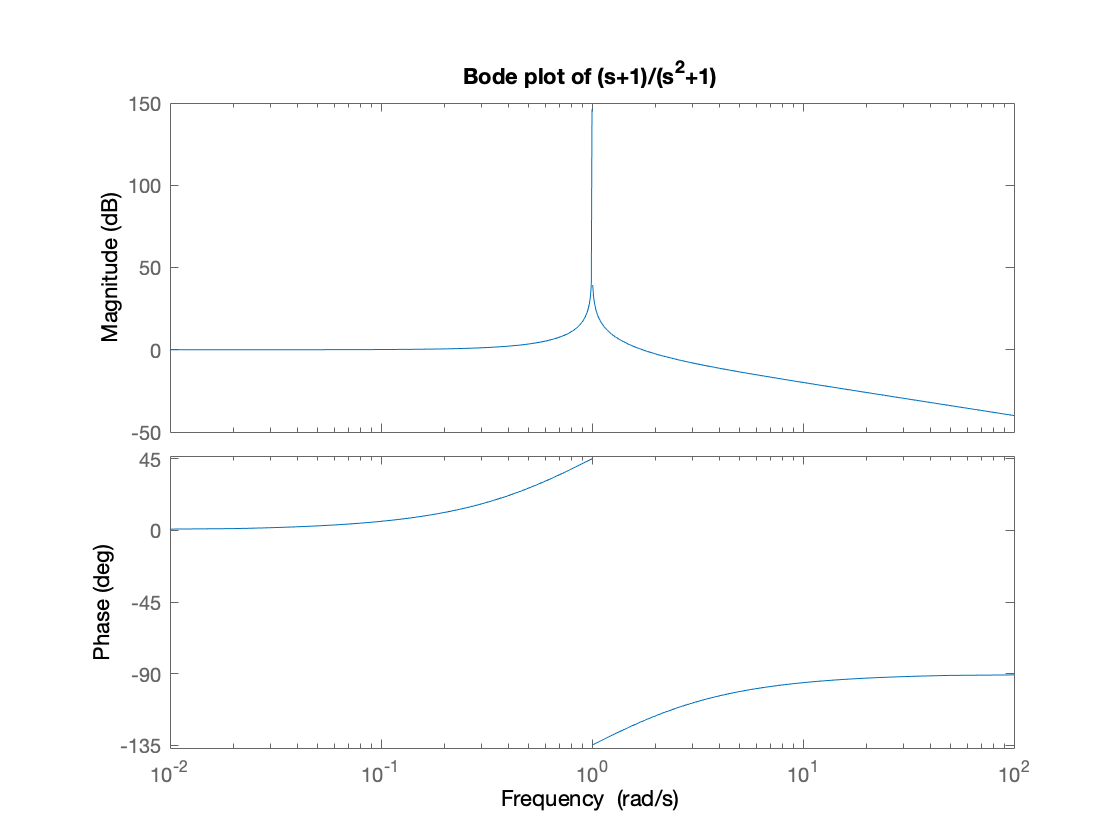
\includegraphics[width=\textwidth]{pic/13.png}
\end{minipage}
\begin{minipage}[t]{0.48\textwidth}
\centering
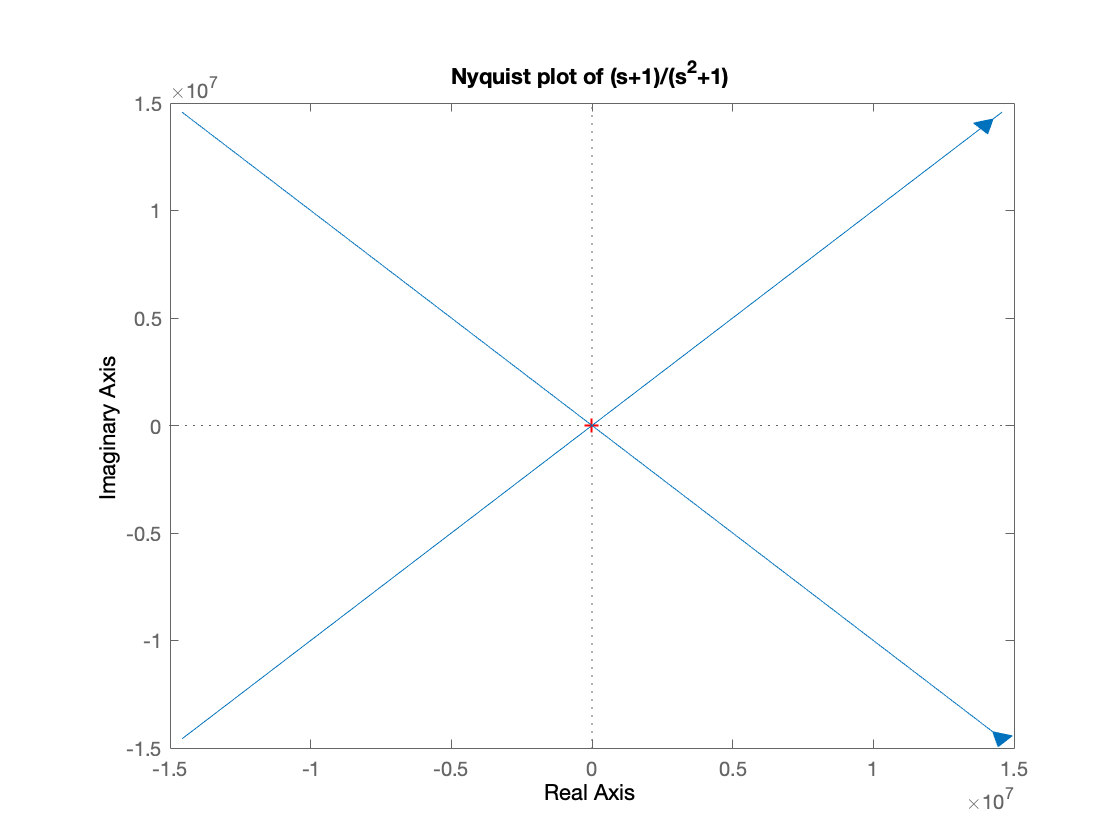
\includegraphics[width=\textwidth]{pic/14.png}
\end{minipage}
\end{figure}
It's stable while in close loop even if crank $K$ up to infinity.

\end{document}